\documentclass[a4paper, 12pt]{extarticle}

% Includes 
\usepackage[utf8]{inputenc} % UTF-8 encode 
\usepackage[english, russian]{babel}
\usepackage{geometry} % adjust page layout 
\usepackage{graphicx} 
\usepackage{hyperref} 
\usepackage{amsmath} % math formulas 
\usepackage{setspace} % for set line spacing 
\usepackage{indentfirst} % indent on a first line after the paragraph 
% \usepackage{pgfplots} % for plots 
\usepackage{xcolor} % colors (used for listings)
\usepackage{listings} % for code listings 
\usepackage{sourcecodepro} % for another monospaced font 
\usepackage{float}

% debug
% \usepackage{showframe} % frame borders for demonstration 


%%% Custom commands
% commands for unnumbered sections
\newcommand{\usection}[1]{\section*{#1} \addcontentsline{toc}{section}{\protect\numberline{}#1}}
\newcommand{\usubsection}[1]{\subsection*{#1} \addcontentsline{toc}{subsection}{\protect\numberline{}#1}}
\newcommand{\usubsubsection}[1]{\subsubsection*{#1} \addcontentsline{toc}{subsubsection}{\protect\numberline{}#1}}


% Redefinition of section and subsection numbering style
\def\thesection{\arabic{section}.}
\def\thesubsection{\arabic{section}.\arabic{subsection}.}
\def\thesubsubsection{\arabic{section}.\arabic{subsection}.\arabic{subsubsection}.}



% Settings for links 
\hypersetup{
    colorlinks=true, % turn ob links coloring 
    citecolor=black, % 
    filecolor=black, % links to local files
    linkcolor=black, % Internal links, those generated by cross-referenced elements
    urlcolor=blue, % links to web sites 
}


% Layout
\geometry{
	left=17mm,
	top=17mm,
	right=17mm,
	bottom=20mm,
	marginparsep=0mm,
	marginparwidth=0mm,
	headheight=8mm,
	headsep=5mm, 
}

\linespread{1.5} % line spacing
\setlength{\parskip}{\baselineskip}  % Add space between paragraphs


% overfull hbox settings
\tolerance 10000 % default 200, max 10000
\hbadness 10000 % default 1000, max 10000
\emergencystretch 0pt  % default 0pt, how much the lines can stretch for the sake of good line breaks
\hfuzz 0.4pt % ignore overfull box less than 
\widowpenalty=10000 % no lines at the start of the page
\vfuzz \hfuzz % don't care about underfull vbox if overfull is acceptable
\raggedbottom % if the page is not filled, align the content to the bottom


% Redefinition of table of contents command to get centered heading
\makeatletter
\renewcommand\tableofcontents{ 
  \begin{singlespace}
    \null\hfill\textbf{\Large\contentsname}\hfill\null\par
    \@mkboth{\MakeUppercase\contentsname}{\MakeUppercase\contentsname}%
    \@starttoc{toc}
  \end{singlespace}
}
\makeatother


% Listings settings
\definecolor{codegreen}{rgb}{0, 0.6, 0}
\definecolor{codegray}{rgb}{0.5, 0.5, 0.5}
\definecolor{codepurple}{rgb}{0.58, 0, 0.82}
\definecolor{backcolour_gray}{rgb}{0.98, 0.98, 0.98}

\lstdefinestyle{python_white}{
  language=Python,
  backgroundcolor=\color{backcolour_gray},   
  commentstyle=\color{codegreen},
  keywordstyle=\color{blue},
  numberstyle=\tiny\color{codegray},
  stringstyle=\color{codepurple},
  basicstyle=\ttfamily\small\singlespacing,
  breakatwhitespace=true,         
  breaklines=true,                 
  captionpos=b, % t/b                  
  keepspaces=true,                 
  numbers=none, % none/left/right                    
  numbersep=5pt,                  
  showspaces=false,                
  showstringspaces=false,
  showtabs=false,                  
  tabsize=2,
  frame=single, % none/leftline/topline/bottomline/lines/single/shadowbox
  rulecolor=\color{gray}, % frame color 
}


\lstset{style=python_white}


% For title page
\def\name{Отчет по лабораторной работе №1} 
\def\subname{Гистограммы, профили, проекции}
\def\madeby{Александр Иванов, Ф ТЕХ.ЗРЕНИЕ 1.1 \\ Ани Аракелян, ТЕХ.ЗРЕНИЕ 1.1\\ Никита Братушка, ТЕХ.ЗРЕНИЕ 1.3}
\def\teacher{Шаветов С. В.}

\begin{document}

% Title page 
\begin{titlepage}

\thispagestyle{empty}

\title{

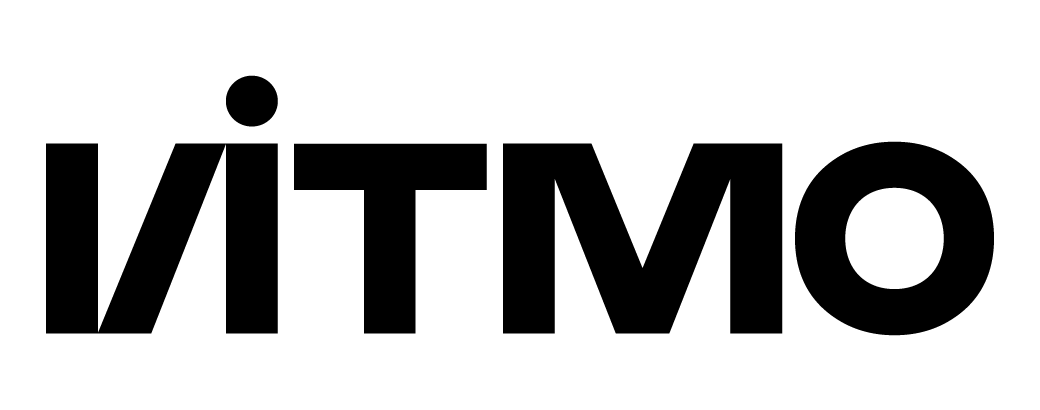
\includegraphics[width=4cm]{media/ITMO_logo.png} 

\vspace{1em}
НИУ ИТМО 
\vspace{4em}

\begin{center}
\large\textsc{\textbf{\name}}

\vspace{1em}
``\subname'' 

\end{center}

\vspace{3em}

\begin{flushright}
\normalsize{ 
Выполнил: \\ \textbf{\madeby} 

Преподаватель: \\ \textbf{\teacher} 
}
\end{flushright}	

\vfill

\begin{center}
\small{Санкт-Петербург, \the\year}
\end{center}
}


\author{}
\date{}
\maketitle
\thispagestyle{empty}
\end{titlepage} % Title page

\addtocounter{page}{1} % Inc counter to start from 2 
\tableofcontents % Table of contents
\pagebreak

\section{Используемые функции}

\subsection{Функция для вычисления гистограммы изображения}

Для вычисления гистограммы изображений была написана следующая функция:

\begin{lstlisting}

def calc_hist_normalised(img):
  histSize = 256
  histRange = (0, 256)
  # calculate the histograms
  b_hist = cv2.calcHist([img], [0], None, [histSize], histRange) / (img.shape[0] * img.shape[1])
  g_hist = cv2.calcHist([img], [1], None, [histSize], histRange) / (img.shape[0] * img.shape[1])
  r_hist = cv2.calcHist([img], [2], None, [histSize], histRange) / (img.shape[0] * img.shape[1])

  return b_hist, g_hist, r_hist
\end{lstlisting}

В качестве аргумента она принимает изображение, для которого необходимо вычислить гистограмму. Возвращает функция нормализованные гистограммы для каждого канала изображения.
Под нормализованной гистограммой понимается гистограмма, в которой каждое значение поделено на общее количество пикселей в изображении.

\subsection{Функция для отображения изображения и его гистограмм}
Для отображения изображения, его гистограмм и результата преобразования использовалась следующая функция: 

\begin{lstlisting}[language=Python]
# add histogram and image to the same plot
def show_image_with_hist(img, title="Image"):
  img_rgb = cv2.cvtColor(img, cv2.COLOR_BGR2RGB) # normal colors to display
  b_hist, g_hist, r_hist = calc_hist_normalised(img) # calculate the histograms
  cumulative_hist_b,cumulative_hist_g, cumulative_hist_r = np.cumsum(b_hist), np.cumsum(g_hist), np.cumsum(r_hist) # calculate the cumulative histograms

  gs = plt.GridSpec(2, 4, width_ratios=[3, 1, 1, 1])

  plt.figure(figsize=(13, 5))

  plt.suptitle(title, fontsize=16)
  ax0 = plt.subplot(gs[:, 0]) # for image 
  ax0.set_title('Image')
  ax1 = plt.subplot(gs[0, 1:4]) # for rgb hist
  ax1.set_title('RGB Histogram')

  ax2 = plt.subplot(gs[1, 1:3])
  ax2.set_title('Cumulative RGB Histogram')
  ax3 = plt.subplot(gs[1, 3])
  ax3.set_title('Average Histogram')

  # set the x axis limits for the histogram subplots and grid
  for ax in [ax1, ax2, ax3]:
      ax.set_xlim([0, 256])
      ax.grid(True)

  # display the image
  ax0.imshow(img_rgb)
  ax0.axis('off')

  # all 3 histograms
  ax1.plot(b_hist, color='b')
  ax1.plot(g_hist, color='g')
  ax1.plot(r_hist, color='r')

  # cumulative histograms
  ax2.plot(cumulative_hist_b, color='b')
  ax2.plot(cumulative_hist_g, color='g')
  ax2.plot(cumulative_hist_r, color='r')

  # add 3 colors hist
  avg_hits = (b_hist + g_hist + r_hist) / 3
  ax3.hist(np.arange(0, 256), bins=256, weights=avg_hits, color='black')

  # adjust the layout
  plt.subplots_adjust(wspace=0.3, hspace=0.3)
  plt.subplots_adjust(left=0.05, right=0.95)  
\end{lstlisting}

Во всех следующих функциях для преобразования изображений оно сначала раскладывается на каналы, затем преобразование применяется к каждому каналу, после чего каналы собираются обратно в изображение. 
В некоторых случаях это позволяет применить различные значения преобразования к различным каналам изображения, что позволяет получить более интересные результаты.

\section{Преобразования изображений}

\subsection{Исходное изображение}

\begin{figure}[H]
    \centering
    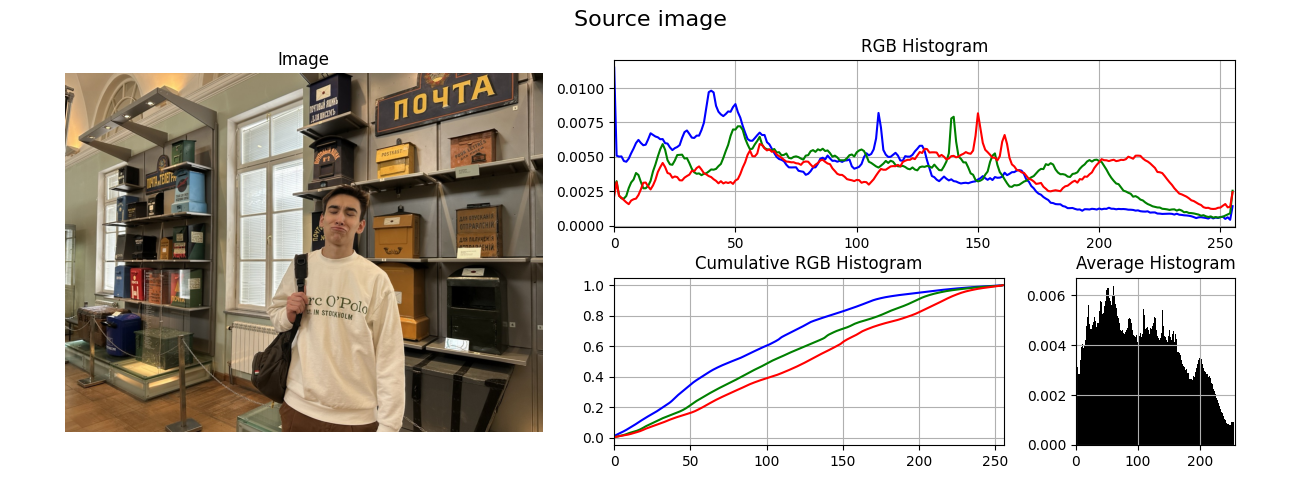
\includegraphics[width=\textwidth]{../results/Source image.png}
    \caption{Исходное изображение}
    \label{fig:source}
\end{figure}

На рисунке \ref{fig:source} представлено исходное изображение, с которым мы будем работать дальше. По гистограмме видно, что на изображении отсутвуют темные и светлые пиксели. 

Кроме того, в правой части рисунка \ref{fig:source} представлены гистограммы для каждого канала изображения, коммулятивная гистограмма и средняя гистограмма для всех каналов.

\subsection{Линейное выравнивание гистограммы}

Суть линейного выравнивания гистограммы заключается в использовании коммулятивнной гистограммы для вычисления нового значения пикселя.

Исходный код функции для линейного выравнивания гистограммы:

\begin{lstlisting}[language=Python]
def linear_leveling_transformation(img):
  # split the image into its 3 channels
  b, g, r = cv2.split(img)

  # calculate the histograms
  hist = calc_hist_normalised(img)

  # calculate the cumulative histograms
  cumulative_histogram_b = np.cumsum(hist[0]) 
  cumulative_histogram_g = np.cumsum(hist[1])
  cumulative_histogram_r = np.cumsum(hist[2])

  # apply the transformation
  b = np.clip(255 * cumulative_histogram_b[b], 0, 255)
  g = np.clip(255 * cumulative_histogram_g[g], 0, 255)
  r = np.clip(255 * cumulative_histogram_r[r], 0, 255)

  # merge the channels back
  return cv2.merge([b, g, r]).astype(np.uint8)
\end{lstlisting}

\begin{figure}[H]
    \centering
    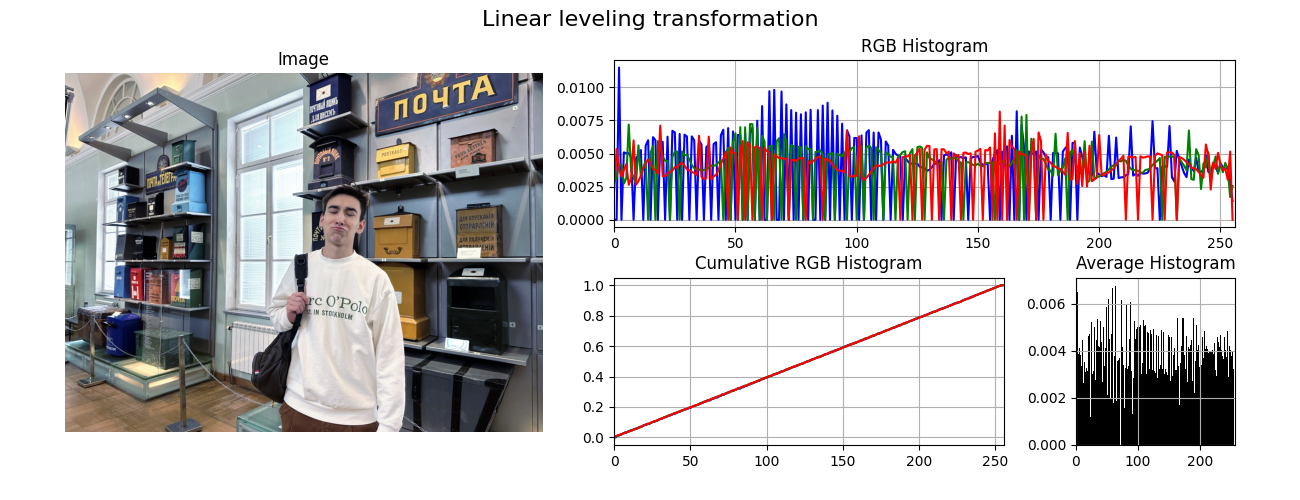
\includegraphics[width=\textwidth]{../results/Linear leveling transformation.png}
    \caption{Результат линейного выравнивания гистограммы}
    \label{fig:linear}
\end{figure}

На рисунке \ref{fig:linear} представлен результат применения линейного выравнивания гистограммы к исходному изображению. Как видно, коммулятивная гистограмма стала представлять из себя линейную функцию, что и является результатом применения линейного выравнивания гистограммы. 

Цвета изображения при этом стали более холодными, сама гистограмма стала прерывистой, что связано с тем, что на преобразованном изображении не могут появиться некоторые значения пикселей. 

Контрастность изображения выросла, так как теперь присутствуют пиксели темных и светлых тонов, которые отсутствовали на исходном изображении. 

\subsection{Арифетические операции над изображениями}

Для увеличения детализации некоторых областей изображения, можно использовать арифметические операции над изображениями. Например, для увеличения детализации теней можно использовать смещение цветов изображения в сторону светлых тонов.

Исходный код функции для арифметических операций над изображениями:

\begin{lstlisting}[language=Python]
def aritmetic_transformation(img, b_delta, g_delta, r_delta):
  # split the image into its 3 channels
  b, g, r = cv2.split(img)

  # add the delta to each channel and divide by 255
  b = np.clip((b + b_delta), 0, 255) 
  g = np.clip((g + g_delta), 0, 255) 
  r = np.clip((r + r_delta), 0, 255) 

  # merge the channels back
  return cv2.merge([b, g, r])
\end{lstlisting}


Так как мы используем цветное изображение, то для каждого канала можно использовать свой коэффициент смещения.

\begin{figure}[H]
    \centering
    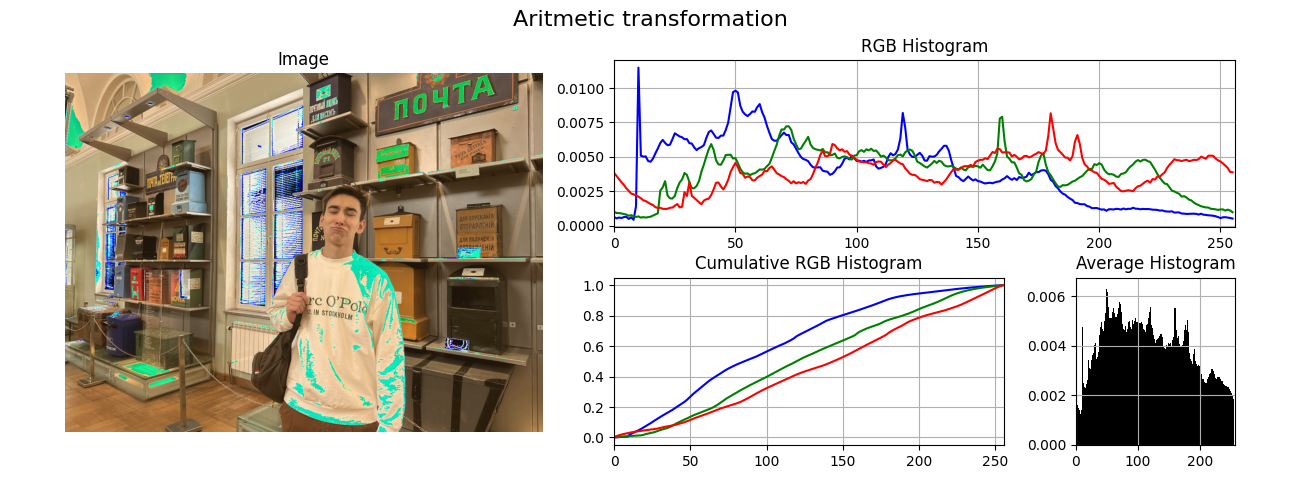
\includegraphics[width=\textwidth]{../results/Aritmetic transformation.png}
    \caption{Результат арифметических операций над изображением}
    \label{fig:aritmetic}
\end{figure}

На рисунке \ref{fig:aritmetic} представлен результат применения арифметических операций над изображением. К красному, зеленому и синему каналам изображения были добавлены значения 30, 20 и 10 соответственно.

Как видно, изображение стало более светлым, что связано с тем, что мы добавили ко всем каналам изображения некоторое значение. На изображении стал преобладать красный цвет, ведь к его значению мы прибавили наибольшее значение. 
Контрастность каждого канала по отдельности при этом не иземенилась, ведь диапазон между самым яарким с самым темным пикселем остался неизменным. 

На гистограмме так же видно, что на изображении стало больше светлых пикселей. 

\subsection{Растяжение динамического диапазона}

Данное преобразование выполняется согласно следующему закону: 

\begin{equation}
  I_{new} = \left( \frac{I - I_{min}}{I_{max} - I_{min}} \right)^\alpha
\end{equation}

где $I$ -- исходное изображение, $I_{new}$ -- преобразованное изображение, $I_{min}$ и $I_{max}$ -- минимальное и максимальное значение пикселя на изображении, $\alpha$ -- коэффициент нелинейности.

Исходный код функции для растяжения динамического диапазона:

\begin{lstlisting}[language=Python]
def dynamic_range_expansion_transformation(img, aplha):
  # find maximum and minimum values for each channel

  # if the image is of type uint8, convert it to float64
  if img.dtype == 'uint8':
      img_converted = img.astype(np.float64) / 255

  b, g, r = cv2.split(img_converted)
  b_min, b_max = b.min(), b.max()
  g_min, g_max = g.min(), g.max()
  r_min, r_max = r.min(), r.max()

  # apply the transformation
  b = np.clip(((b - b_min) / (b_max - b_min)) ** aplha, 0, 1)
  g = np.clip(((g - g_min) / (g_max - g_min)) ** aplha, 0, 1)
  r = np.clip(((r - r_min) / (r_max - r_min)) ** aplha, 0, 1)

  img_transformed = cv2.merge([b, g, r]) # merge the channels back

  # convert the image back to uint8 if it was initially of that type
  if img.dtype == 'uint8':
      img_transformed = (255 * img_transformed).clip(0, 255).astype(np.uint8)

  return img_transformed
\end{lstlisting}

\begin{figure}[H]
    \centering
    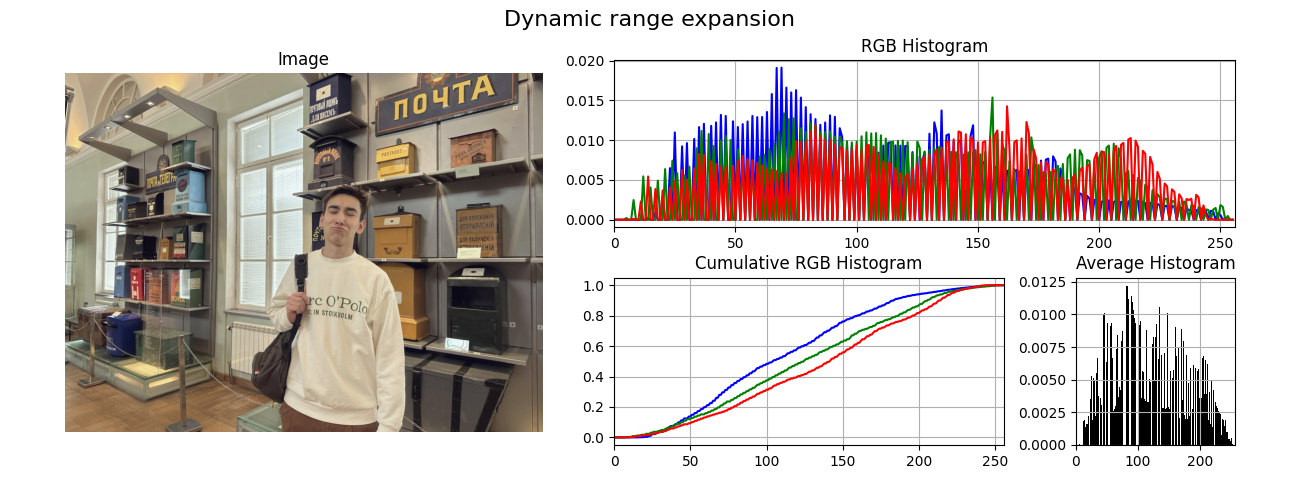
\includegraphics[width=\textwidth]{../results/Dynamic range expansion.png}
    \caption{Результат растяжения динамического диапазона}
    \label{fig:dynamic}
\end{figure}

На рисунке \ref{fig:dynamic} представлен результат применения растяжения динамического диапазона к исходному изображению. Как видно, изображение стало более контрастным. 
Гистограмма как-будто \textit{растянулась}, теперь на изображении присутствуют как самые светлые, так и самые темные пиксели. 

\subsection{Равномерное преобразование}

Равномерное преобразование выполняется согласно следующему закону:

\begin{equation}
  I_{new} = \left( I_{max} - I_{min} \right) * P(I) + I_{min}
\end{equation}

где $I$ -- исходное изображение, $I_{new}$ -- преобразованное изображение, $I_{min}$ и $I_{max}$ -- минимальное и максимальное значение пикселя на изображении, $P(I)$ -- функция распределения вероятностей исходного изображения, которая аппроксимируется коммулятивнной гистограммой: 

\begin{equation}
  P(I) \approx \sum\limits_{m=0}^{i} Hist(m)
\end{equation}

Исходный код функции для равномерного преобразования:

\begin{lstlisting}[language=Python]
def uniform_transformation(img):
  b, g, r = cv2.split(img)
  # calculate the histograms
  hist = calc_hist_normalised(img)

  b_min, b_max = b.min(), b.max()
  g_min, g_max = g.min(), g.max()
  r_min, r_max = r.min(), r.max()

  cumulative_histogram_b = np.cumsum(hist[0]) 
  cumulative_histogram_g = np.cumsum(hist[1])
  cumulative_histogram_r = np.cumsum(hist[2])

  b = np.clip((b_max - b_min) * cumulative_histogram_b[b] + b_min, 0, 255)
  g = np.clip((g_max - g_min) * cumulative_histogram_g[g] + g_min, 0, 255)
  r = np.clip((r_max - r_min) * cumulative_histogram_r[r] + r_min, 0, 255)

  return cv2.merge([b, g, r]).astype(np.uint8)
\end{lstlisting}

\begin{figure}[H]
    \centering
    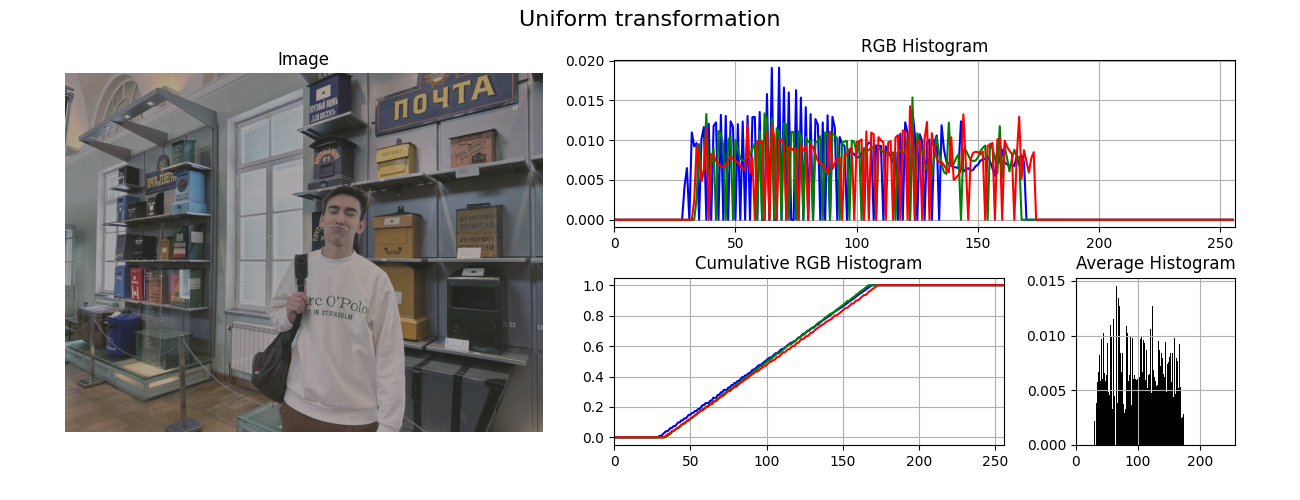
\includegraphics[width=\textwidth]{../results/Uniform transformation.png}
    \caption{Результат равномерного преобразования}
    \label{fig:uniform}
\end{figure}

На рисунке \ref{fig:uniform} представлен результат применения равномерного преобразования к исходному изображению. 
Как видно, изображение стало более контрастным, при этом коммулятивнная гистограмма стала представлять из себя
линейную функцию (на отрезке), что схоже с результатом применения линейного выравнивания гистограммы, но 
в данном случае не произошло \textit{растяжение} гистограммы, а выравнивание проихошло только в исходном диапазоне. 


\subsection{Экспоненциальное преобразование}

Экспоненциальное преобразование выполняется согласно следующему закону:

\begin{equation}
  I_{new} = I_min - \frac{1}{\alpha} \cdot \ln(1 - P(I))
\end{equation}

где $I$ -- исходное изображение, $I_{new}$ -- преобразованное изображение, $I_{min}$ -- минимальное значение пикселя на изображении, $P(I)$ -- функция распределения вероятностей исходного изображения, $\alpha$ -- постоянная, характеризующая крутизну преобразования. 

Исходный код функции для экспоненциального преобразования:

\begin{lstlisting}[language=Python]
def exponentional_transformation(img, alpha):
  b, g, r = cv2.split(img)
  # calculate the histograms
  hist = calc_hist_normalised(img)

  b_min, b_max = b.min(), b.max()
  g_min, g_max = g.min(), g.max()
  r_min, r_max = r.min(), r.max()

  cumulative_histogram_b = np.cumsum(hist[0]) 
  cumulative_histogram_g = np.cumsum(hist[1])
  cumulative_histogram_r = np.cumsum(hist[2])

  b = b_min - 255/alpha * np.log(1 - cumulative_histogram_b[b]) 
  g = g_min - 255/alpha * np.log(1 - cumulative_histogram_g[g]) 
  r = r_min - 255/alpha * np.log(1 - cumulative_histogram_r[r]) 

return (cv2.merge([b, g, r])).astype(np.uint8).clip(0, 255)
\end{lstlisting}

\begin{figure}[H]
    \centering
    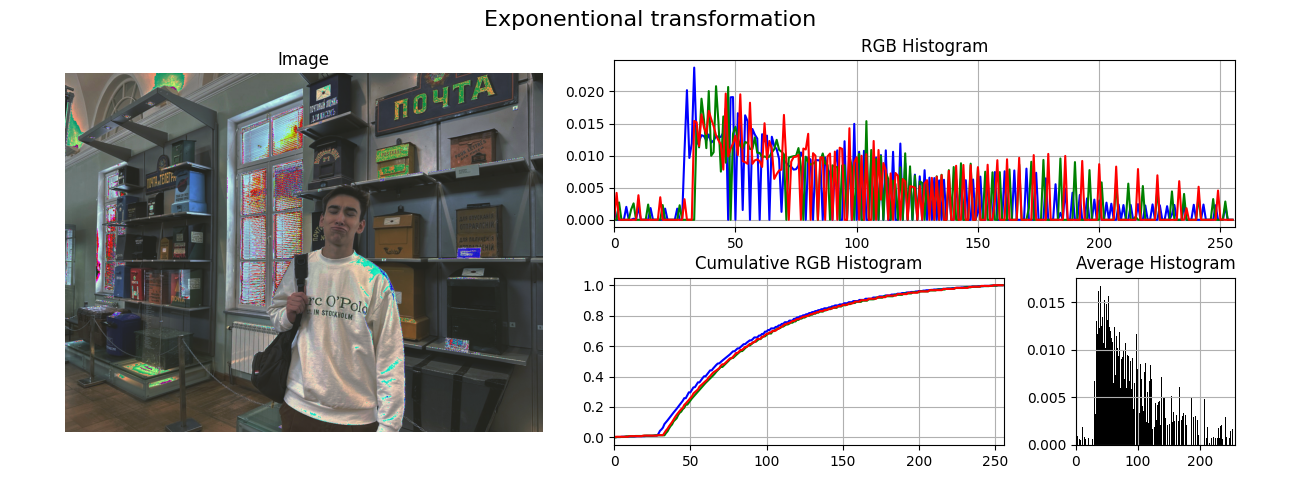
\includegraphics[width=\textwidth]{../results/Exponentional transformation.png}
    \caption{Результат экспоненциального преобразования}
    \label{fig:exponentional}
\end{figure}

На рисунке \ref{fig:exponentional} видим, что график коммулятивнной гистограммы действительно стал представлять из себя экспоненциальную функцию. 
При этом начало графика коммулятивной гистораммы является горизонтальной прямой. Это связано с тем, что на изображении отсутствовали темные пиксели. 

При этом изображение стало значительно темнее, что так же видно на гистограммах -- темные пиксели стали преобладать на изображении.


\subsection{Преобразование по закону Рэлея}  

Преобразование по закону Рэлея выполняется согласно следующему закону:

\begin{equation}
  I_{new} = I_{min} + \left(2\alpha^2 \cdot \ln\left(\frac{1}{1 - P(I)}\right)\right)
\end{equation}

где $\alpha$ -- постоянная, характеризующая гистограмму распределения интенсивностей элементов результирующего изображения. 

Исходный код функции для преобразования по закону Рэлея:

\begin{lstlisting}[language=Python]
def rayleigh_law_transformation(img, alpha):
  b, g, r = cv2.split(img)
  # calculate the histograms
  hist = calc_hist_normalised(img)

  b_min, b_max = b.min(), b.max()
  g_min, g_max = g.min(), g.max()
  r_min, r_max = r.min(), r.max()

  cumulative_histogram_b = np.cumsum(hist[0]) 
  cumulative_histogram_g = np.cumsum(hist[1])
  cumulative_histogram_r = np.cumsum(hist[2])

  b = np.clip(b_min + (2*alpha**2 * np.log(1 / (1 - cumulative_histogram_b[b]))) ** 0.5 * 255, 0, 255)
  g = np.clip(g_min + (2*alpha**2 * np.log(1 / (1 - cumulative_histogram_g[g]))) ** 0.5 * 255, 0, 255)
  r = np.clip(r_min + (2*alpha**2 * np.log(1 / (1 - cumulative_histogram_r[r]))) ** 0.5 * 255, 0, 255)
  
  return cv2.merge([b, g, r]).astype(np.uint8)
\end{lstlisting}

\begin{figure}[H]
    \centering
    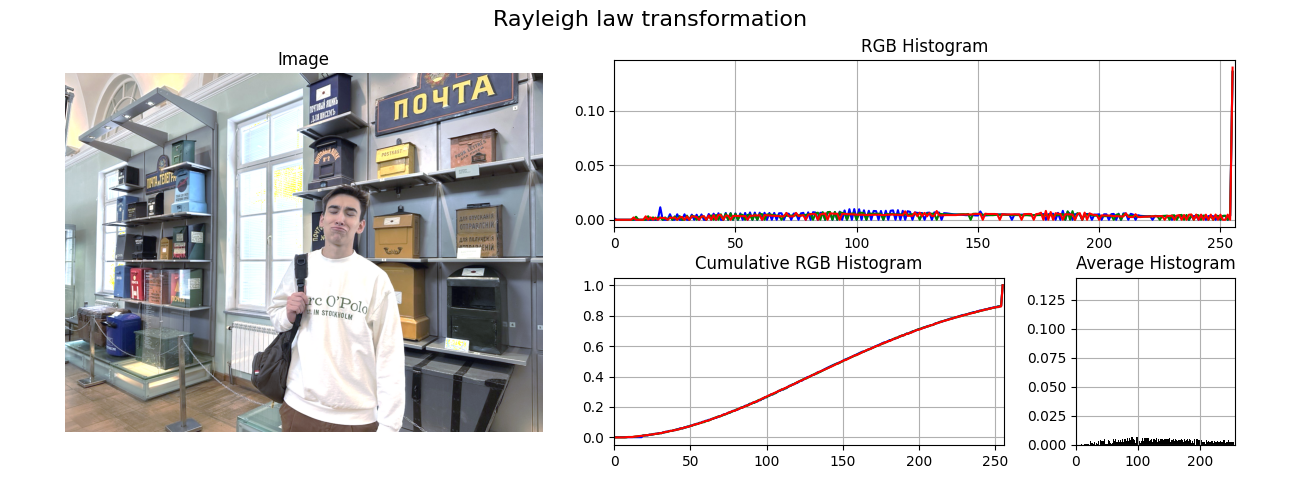
\includegraphics[width=\textwidth]{../results/Rayleigh law transformation.png}
    \caption{Результат преобразования по закону Рэлея}
    \label{fig:rayleigh}
\end{figure}

На рисунке \ref{fig:rayleigh} видим, что график коммулятивнной гистограммы действительно стал представлять из себя функцию Рэлея. Так же наблюдаем сильное преобладание светлых пикселей на изображении. 

\subsection{Преобразование по закону степени 2/3}

Преобразование по закону степени 2/3 выполняется согласно следующему закону:

\begin{equation}
  I_{new} = P(I)^{\frac{3}{2}}
\end{equation}

Исходный код функции для преобразования по закону степени 2/3:

\begin{lstlisting}[language=Python]
def two_thirds_rule_transformation(img):
  b, g, r = cv2.split(img)
  # calculate the histograms
  hist = calc_hist_normalised(img)

  b_min, b_max = b.min(), b.max()
  g_min, g_max = g.min(), g.max()
  r_min, r_max = r.min(), r.max()

  cumulative_histogram_b = np.cumsum(hist[0]) 
  cumulative_histogram_g = np.cumsum(hist[1])
  cumulative_histogram_r = np.cumsum(hist[2])

  b = np.clip((cumulative_histogram_b[b] ** (2/3) * 255), 0, 255)
  g = np.clip((cumulative_histogram_g[g] ** (2/3) * 255), 0, 255)
  r = np.clip((cumulative_histogram_r[r] ** (2/3) * 255), 0, 255)
  
  return cv2.merge([b, g, r]).astype(np.uint8)
\end{lstlisting}

\begin{figure}[H]
    \centering
    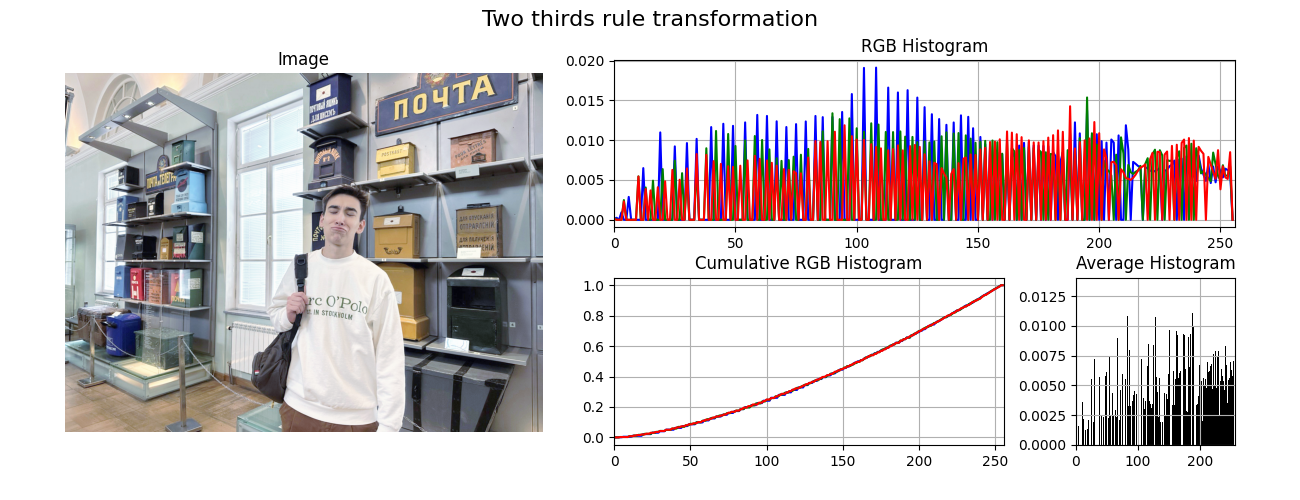
\includegraphics[width=\textwidth]{../results/Two thirds rule transformation.png}
    \caption{Результат преобразования по закону степени 2/3}
    \label{fig:two_thirds}
\end{figure}

На рисунке \ref{fig:two_thirds} видим, что график коммулятивнной гистограммы действительно стал представлять из себя функцию степени 2/3. 

Изображение стало намного более светлым, контрастность вырасла. 

\subsection{Гиперболическое преобразование}  

Гиперболическое преобразование выполняется согласно следующему закону:

\begin{equation}
  I_{new} = \alpha^{P(I)}
\end{equation}

где $\alpha$ -- постоянная, относительно которой осуществляется преобразование.

Исходный код функции для гиперболического преобразования:

\begin{lstlisting}[language=Python]
def hyperbolic_transformation(img, alpha):
  b, g, r = cv2.split(img)
  # calculate the histograms
  hist = calc_hist_normalised(img)

  b_min, b_max = b.min(), b.max()
  g_min, g_max = g.min(), g.max()
  r_min, r_max = r.min(), r.max()

  cumulative_histogram_b = np.cumsum(hist[0]) 
  cumulative_histogram_g = np.cumsum(hist[1])
  cumulative_histogram_r = np.cumsum(hist[2])

  b = np.clip(alpha ** cumulative_histogram_b[b] * 255, 0, 255)
  g = np.clip(alpha ** cumulative_histogram_g[g] * 255, 0, 255)
  r = np.clip(alpha ** cumulative_histogram_r[r] * 255, 0, 255)
  
  return cv2.merge([b, g, r]).astype(np.uint8)
\end{lstlisting}

\begin{figure}[H]
    \centering
    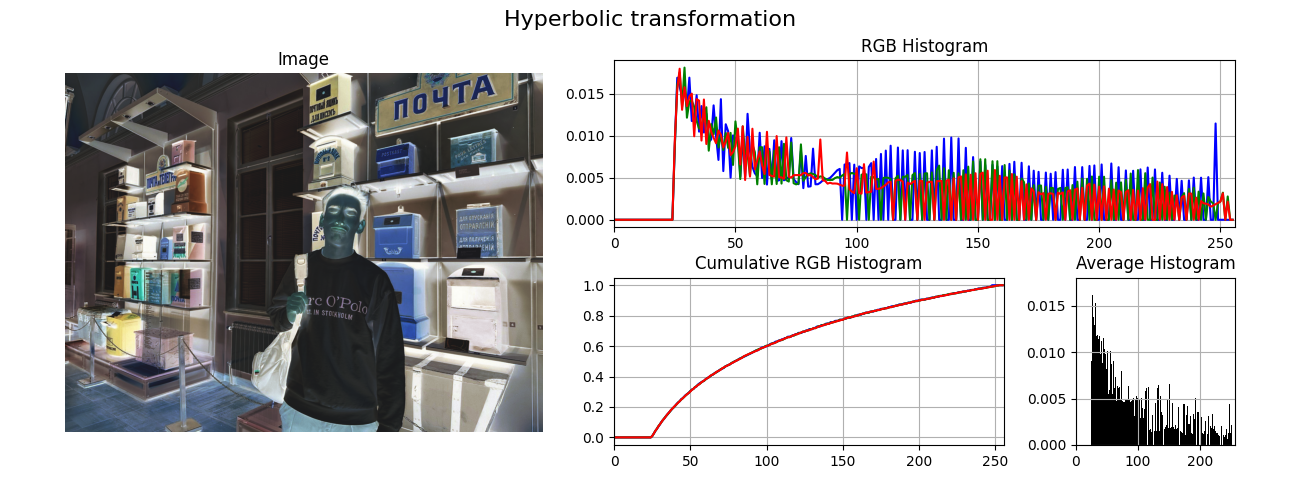
\includegraphics[width=\textwidth]{../results/Hyperbolic transformation.png}
    \caption{Результат гиперболического преобразования}
    \label{fig:hyperbolic}
\end{figure}

На рисунке \ref{fig:hyperbolic} видим, что график коммулятивнной гистограммы изменился, при этом начало графика представляет их себя горизонтальную
прямую. Это связано с тем, что на исходном изображении отсутствовали темные пиксели. 

Изображение можно описать как негативное от исходонго, заметно явное преобладание темных пикселей на изображении.

\subsection{Таблица поиска}

Таблица поиска (lookup table) -- это таблица, в которой для каждого значения пикселя изображения задается новое значение пикселя.

Исходный код функции для преобразования по таблице поиска:

\begin{lstlisting}[language=Python]
def LUT_transformation(img, LUT):
  return cv2.LUT(img, LUT).astype(np.uint8)
\end{lstlisting}

Для создания самой таблицы поиска использовался следующий код:  

\begin{lstlisting}[language=Python]
# generate LUT 
lut = np.arange(256, dtype = np.uint8)
lut = np.clip(np.power(lut, 0.9) + 20, 0, 255)
\end{lstlisting}

\begin{figure}[H]
    \centering
    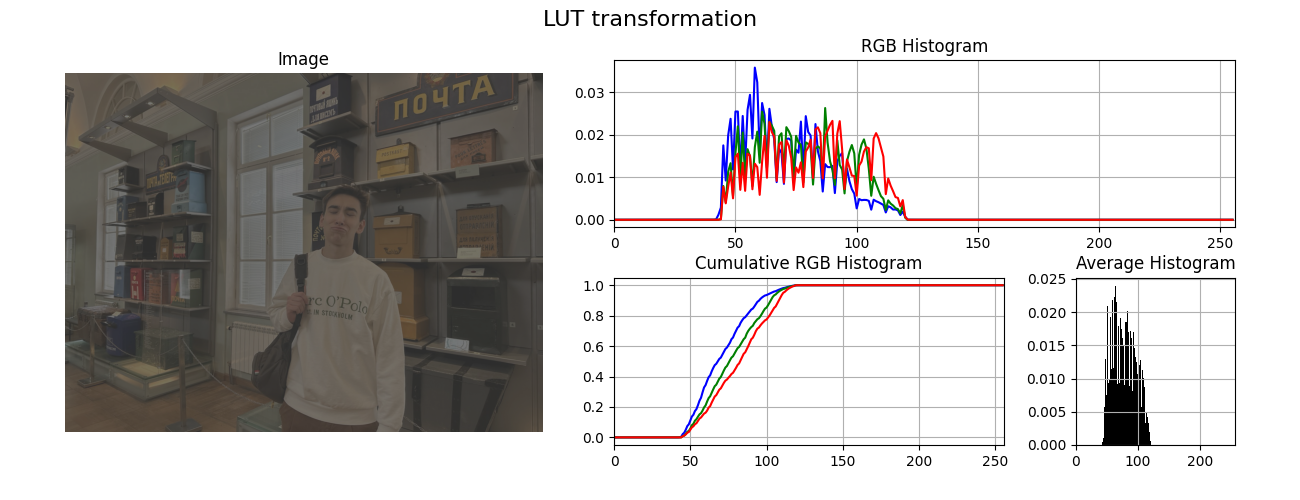
\includegraphics[width=\textwidth]{../results/LUT transformation.png}
    \caption{Результат преобразования по таблице поиска}
    \label{fig:lut}
\end{figure}

На рисунке \ref{fig:lut} видим, что график коммулятивнной гистограммы стал представлять из себя функцию степени 0.9, смешение на 20, что и было задано в таблице поиска.  

\section{Профили изображения}

Профилем изображения вдоль некоторой линии называется функция интенсивности изображения, распределенного вдоль этой линии (\textit{прорезки}).

Рассмотрим профили изображения вдоль горизонтальной и вертикальной линий: 

\begin{equation}
  Profile~i(x) = I(x, i)
\end{equation}
  
\begin{equation}
  Profile~i(y) = I(i, y)
\end{equation}

где $I(x, i)$ -- интенсивность пикселя изображения в точке $(x, i)$, $I(i, y)$ -- интенсивность пикселя изображения в точке $(i, y)$.

\subsection{Профиль изображения вдоль горизонтальной линии}

Рассмотрим профиль изображения со штрих-кодом вдоль горизонтальной линии.

Исходный код функции для вычисления профиля изображения вдоль горизонтальной линии:

\begin{lstlisting}[language=Python]
def show_image_profile(img, level):
  img_rgb = cv2.cvtColor(img, cv2.COLOR_BGR2RGB) # normal colors to display
  plt.figure(figsize=(13, 5))
  plt.subplot(1, 2, 1)
  plt.title('Image')
  plt.imshow(img_rgb)
  plt.axis('off') # disable the axis

  plt.subplot(1, 2, 2)
  profile = img[level, :]
  plt.plot(profile)
  plt.title('Profile')

  plt.subplots_adjust(wspace=0.3, hspace=0.3)
  plt.subplots_adjust(left=0.05, right=0.95)

show_image_profile(img, img.shape[0] // 2)
\end{lstlisting}

\begin{figure}[H]
    \centering
    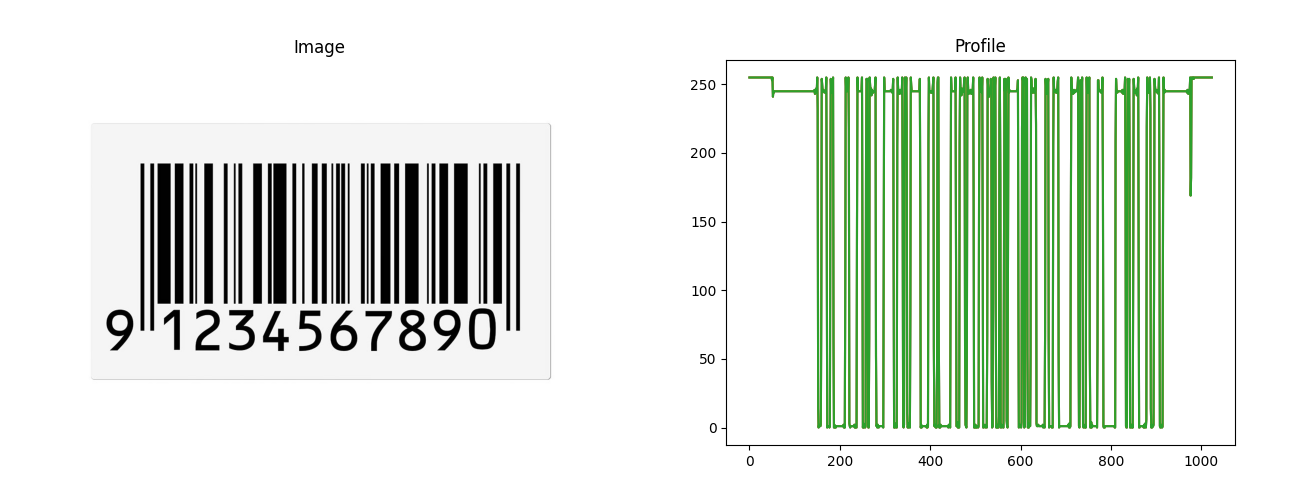
\includegraphics[width=\textwidth]{../results/Profile.png}
    \caption{Профиль изображения вдоль горизонтальной линии}
    \label{fig:profile}
\end{figure}

Видим, что на профиле хорошо различимы  \textit{штрихи} штрих-кода. Данную проекцию можно исопльзовать для распознавания штрих-кода. 

\section{Проекция изображения}

Проекцией изображения на некоторую ось называется сумма интенсивностей пикселей изображения в направлении, перпендикулярном этой оси.

\subsection{Проекция изображения на оси}

Рассмотрим проекцию изображения на горизонтальную и вертикальную оси:

\begin{equation}
  Projection~X(y) = \sum\limits_{i=0}^{dim~Y - 1} I(y, i)
\end{equation}

\begin{equation}
  Projection~Y(x) = \sum\limits_{i=0}^{dim~X - 1} I(i, x)
\end{equation}

Исходный код функции для вычисления проекции изображения на оси:

\begin{lstlisting}[language=Python]
def show_image_projection(img, title="Projection"):
  b, g, r = cv2.split(img)
  # calculate 0x projection
  projection_x = (np.sum(b, axis=0) + np.sum(g, axis=0) + np.sum(r, axis=0)) / img.shape[0] / 3

  # calculate 0y projection
  projection_y = (np.sum(b, axis=1) + np.sum(g, axis=1) + np.sum(r, axis=1)) / img.shape[1] / 3

  plt.figure(figsize=(8, 8))
  plt.subplot(2, 2, 1)
  plt.grid(True)
  plt.title('Image')
  plt.imshow(cv2.cvtColor(img, cv2.COLOR_BGR2RGB))

  plt.subplot(2, 2, 3)
  plt.ylim([255, 0])
  plt.xlim([0, img.shape[1]])
  plt.grid(True)
  plt.plot(range(img.shape[1]), projection_x, color='g')
  plt.title('Projection X')

  plt.subplot(2, 2, 2)
  plt.xlim([0, 255])
  plt.ylim([img.shape[1], 0])
  plt.grid(True)
  plt.plot(projection_y, range(img.shape[0]), color='g')
  plt.title('Projection Y')

  plt.subplots_adjust(wspace=0.3, hspace=0.3)
  plt.subplots_adjust(left=0.05, right=0.95)

  # save image
  plt.savefig(f"results/{title}.png")

show_image_projection(img1, "Projection 1")
show_image_projection(img2, "Projection 2")
\end{lstlisting}

\begin{figure}[H]
    \centering
    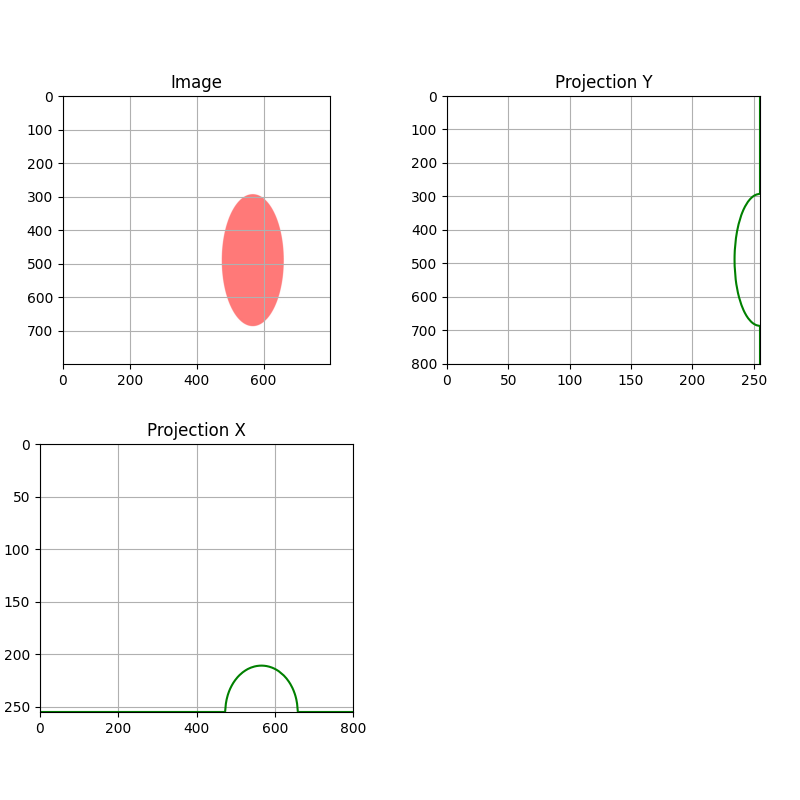
\includegraphics[width=\textwidth]{../results/Projection 1.png}
    \caption{Проекция изображения 1}
    \label{fig:projection1}
\end{figure}

\begin{figure}[H]
    \centering
    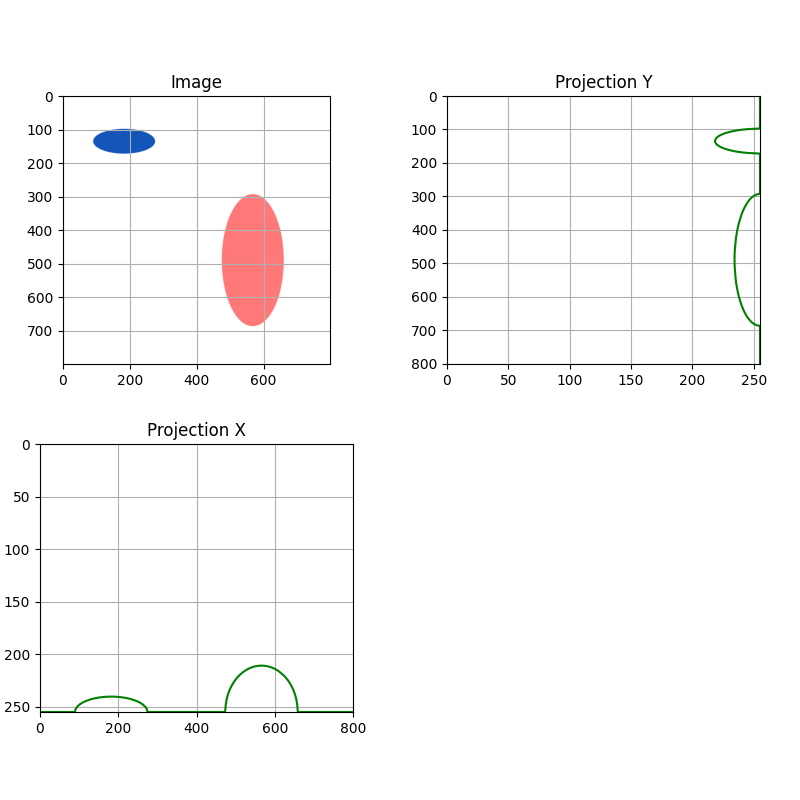
\includegraphics[width=\textwidth]{../results/Projection 2.png}
    \caption{Проекция изображения 2}
    \label{fig:projection2}
\end{figure}

На рисунках \ref{fig:projection1} и \ref{fig:projection2} представлены проекции изображений на горизонтальную и вертикальную оси. 
По этим проекциям можно определить расположение объектов на изображении, а так же их размеры.

\newpage\clearpage
\section{Вывод}

В ходе выполнения лабораторной работы были освоены основные яркостные и геометрические
характеристики изображений и их использование для анализа изображений. 
Мы познакомились с библиотекой \texttt{openCV2}, реализовали преобразования изображений на языке Python. 

Рассмотрев различные преобразования выбранной нами фотографии и полученные гистограммы, мы смогли лучше понять природу данных преобразований. 



Исходный код программы можно найти в \href{https://github.com/edelwiw/TechVision_Lab1}{репозитории на Github.}

\section{Ответы на вопросы}

\newcounter{question}
\setcounter{question}{0}

\newcommand{\question}[1]{\item[Q\refstepcounter{question}\thequestion.] #1}
\newcommand{\answer}[1]{\item[A\thequestion.] #1}

\begin{itemize}

\question{Что такое контрастность изозбражения и как ее можно изменить?}
\answer{Контрастность -- интервал между максимальной и минимальной яркостью пикселей. 
Для изменения контрастности можно использовать различные преобразования изображения, 
в зависимости от исходного изображения и результата, который мы хотим получить,
в том числе, рассмотренные в данной лабораторной работе.

В качестве наглядного примера можно привести преобразование по закону Рэлея (см. рис.~\ref{fig:rayleigh}) или растяжение динамического диапазона (см. рис.~\ref{fig:dynamic})
}
\question{Чем эффективно использование профилей и проекций изображения?}
\answer{С помощью профилей и проекций можно определить расположение объектов на изображении, 
а так же их размеры. Например, это можно использовать для определения позиции текста на изображении и 
дальнейшего его распознавания.}

\question{Каким образом можной найти объект на равномерном фоне?}
\answer{Можно построить проекцию изображения на оси. Анализ массива проекции позволяет выделять 
характерные точки функции проекции, которые соответствуют контурам объектов на изображении. 
Например, если на изображении имеются контрастные объекты, то в проекции будут видны 
перепады или экстремумы функции, соответствующие положению каждого из объектов.}

\end{itemize}



 % Content

\end{document}